\documentclass{article}
\usepackage{amsfonts}
\usepackage{amsthm}
\usepackage{amssymb}
\usepackage{amsmath}
\usepackage{graphicx}
\usepackage{subcaption}
\usepackage{xcolor}
\usepackage{mathtools}
\usepackage{ wasysym }
\usepackage{enumerate}
\usepackage{verbatim}
\usepackage{subcaption}

%Bibliography
\usepackage[backend=biber,style=numeric]{biblatex}
\addbibresource{references.bib}


\newcommand{\new}[2]{
    \vspace{2mm}
    \noindent
    \textbf{
    \underline{#1}}
    \textit{{#2}}
    \
    \newline
}

\def\<{{\langle}}
\def\>{{\rangle}}

\DeclarePairedDelimiter\bra{\langle}{\rvert}
\DeclarePairedDelimiter\ket{\lvert}{\rangle}
\DeclarePairedDelimiterX\braket[2]{\langle}{\rangle}{#1\,\delimsize\vert\,\mathopen{}#2}



\newcounter{problemcnt}
\setcounter{problemcnt}{0}

\newcommand{\Problem}{{
    \vspace{5mm}
    \stepcounter{problemcnt}
    \noindent
    \arabic{problemcnt}. 
}
}

\newcommand{\nProblem}[1]{
    \vspace{5mm}
    \noindent
    \setcounter{problemcnt}{#1}
    \arabic{problemcnt}. 
}


\newcommand{\Proof}{{
    \vspace{2mm}
    \noindent
    \textbf{
    \underline{Proof}}
}
}

\newcommand{\textOr}{
    {
        \hspace{5mm}
        \textrm{or}
        \hspace{5mm}
    }
}

\newcommand{\textAnd}{
    {
        \hspace{5mm}
        \textrm{and}
        \hspace{5mm}
    }
}


\newcommand{\textWhere}{
    {
        \hspace{5mm}
        \textrm{where}
        \hspace{5mm}
    }
}



\newcommand{\Ixp}[1]{
    {
        e^{i{#1}}
    }
}



\newcommand{\halfFigure}[1]{
\begin{center}
\includegraphics[width = .5\linewidth]{{#1}}
\end{center}
}

\newcommand{\fullFigure}[1]{
\begin{center}
\includegraphics[width = .9\linewidth]{{#1}}
\end{center}
}

\def\twobytwoMat(#1, #2, #3, #4){
    {
        \begin{bmatrix}
            {#1} & {#2}\\
            {#3} & {#4}
        \end{bmatrix}
    }
}

\def\twobyoneMat(#1, #2){
    {
        \begin{bmatrix}
            {#1}\\
            {#2}
        \end{bmatrix}
    }
}

\def\twobytwoDet(#1, #2, #3, #4){
    {
        \begin{vmatrix}
            {#1} & {#2}
            {#3} & {#4}
        \end{vmatrix}
    }
}


\newcommand{\RR}{\mathbb{R}}
\newcommand{\CC}{\mathbb{C}}
\newcommand{\ZZ}{\mathbb{Z}}
\newcommand{\Zpos}{\mathbb{Z}_{pos}}
\newcommand{\NN}{\mathbb{N}}

\newtheorem{theorem}{Theorem}[section]
\newtheorem{prop}{Proposition}[section]
\newtheorem{lemma}{Lemma}[section]
\newtheorem{cor}{Corollary}[section]
\newtheorem{remark}{Remark}[section]
\newtheorem{definition}{Definition}[section]
\newtheorem{ex}{Example}[section]
\newtheorem{conj}{Conjecture}[section]
\newtheorem{question}{Question}[section]

\begin{comment}
\newtheorem{theorem}{Theorem}
\newtheorem{prop}{Proposition}
\newtheorem{lemma}{Lemma}
\newtheorem{cor}{Corollary}
\newtheorem{remark}{Remark}
\newtheorem{definition}{Definition}
\newtheorem{ex}{Example}
\newtheorem{conj}{Conjecture}
\newtheorem{question}{Question}
\end{comment}



\numberwithin{equation}{section}



\newcommand{\ch}{\text{ch}}

\begin{document}
\begin{center}
    \Large
    \textbf{Predator-Prey Model using Leslie matricies and optimal predation strategies}

    \large
    PP Group
\end{center}

\tableofcontents

\section{Abstract}

In this paper, we introduce a new predator-prey model based 
the Lotka-Voltera model. Extensive study have been conducted 
on the stability of the equation for the simple model which 
considers an homogenous population
. For example, Merdan carries 
out a stability analysis by computing the Jacobian and 
drawing from methods of differential calculus. 

We replace the population evolution constants 
to a Leslie matrix, taking account of multiple age groups. 
Replacing the constant coefficients to 
Leslie matrices motivates the study of dominant eigenvalues 
which can be conducted using techniques in Complex Analysis. 
Using the theory of dominating eigenvalues, we provide a bound 
for maximum predation rate for population survival in a long term. 
We also discuss the competitive model, and prove the 
last species standing theorem, which describes the unlikelihood 
of stable equilibrium between two competitive species. 

Moreover, we analyze an open population where migration 
is allowed. We first study 
population under constant migration provide conditions for harmonic fluctuations 
of the model. Also, expanding on the work of Arditi 
and Ginzburg, we study the case where migration considered 
as a response to the environment, i.e. dependent on the population. 


\section{Single Species Population}
%simple leslie matrix

\subsection{Definition of Simple Leslie Matricies and the Lotka-Euler Equation}

Leslie matricies characterize the change of population with 
different age groups, given the survival rate and the fertility rate 
of the species. 

%possibly some explanation of Leslie matricies

We focus on a specific class of Leslie matricies with 
a fixed fertility rate $f$ and a survival rate 1. 

\begin{definition}[Simple Leslie Matricies]
    \label{LeslieDef}

    Suppose $N \in \mathbb{Z}_{pos}$. A simple Leslie matrix that 
    characterizes the population evolution is defined as follows. 

    \[
        (L_f)_{ij} = \begin{cases}
            f & (i = 0)\\
            1 & (i \neq 0 \wedge j=i+1)\\
            0 & \textrm{Otherwise}\\
        \end{cases}
    \]
        Or writing the matrix out, 
    \[L_f :=
    \begin{bmatrix}
        f & f& \cdots & f \\ 
        1 & 0 & \cdots & 0 \\
        0 & 1 & \cdots & 0\\
        &&\vdots &\\
        0 & \cdots & 1 & 0
    \end{bmatrix} 
    \]. 
\end{definition}

The maximum eigenvalue of this Matrix describes the asymptotic 
behavior of the population. The first apporach is to compute the characteristic 
equation and find the roots to derive properties about the eigenvalues. 

\begin{theorem}[Lotka-Euler Equation]
    \label{LEeq}
    The characteristic equation of a simple leslie matrix $L_f$ of 
    order $N$ greater than 1 is 
    \[
        \ch_N(x):=x^N - f(x^{N-1} + \cdots + x + 1)
    \]
    which, using the geometric series formula, can be simplified as 
    \[
        x^{N} - f \frac {x^N - 1} {x - 1}
    \]
\end{theorem}

\begin{proof} Induct on N. It is trivial to see that the equation holds for 
$N = 1$. For the inductive step, consider $N > 2$. We write out the 
characteristic polynomial as a determinant expansion. 

\[
    \ch_{N + 1} \ = \ \textrm{det}(xI - L_f) 
    \ = \ 
    \begin{vmatrix}
        x - f & -f& \cdots & -f \\ 
        -1 & x & \cdots & 0 \\
        0 & -1 & \cdots & 0\\
        &&\vdots &\\
        0 & \cdots & -1 & x
    \end{vmatrix} 
\]

Expand the determinant with respect to the last column. 
\[
    \ch_{N + 1}(x) \ = \ 
    (-f)(-1)^N(-1)^N + x\ch_{N}(x)
\]
By the inductive hypothesis, we write 
\[
    \ch_{N + 1}(x) \ = \ 
    -f + x\left(
    x^N - f(x^{N-1} + \cdots + x + 1)
    \right)
    \ = \ 
x^{N + 1} - f(x^{N} + \cdots + x + 1)
\]
which concludes the proof. 
\end{proof}


\subsection{Bounding Maximum Eigenvalue}
To determine population strategies, it is useful to bound the maximum eigenvalues. 
Using methods from Complex Analysis, it is possible to derive the following 
two theorems. 

\begin{theorem}[Complex Roots of the Characteristic Equation]\label{thm:compRoots}
    The characteristic equation $\ch_N(z)$ has exactly one dominating 
    real eigenvalue. All other roots lie inside the unit circle. 
\end{theorem}

\begin{proof}
    We consider the polynomial 
    \[
        \bar h(z) := (z - 1) \ch_N(z) = z^{N+1} - (f + 1)z^N + f
    \]
    and show that all the complex roots lie inside the unit circle. 
    It suffices to show that 
    \[
        h(z) \ :=\ \bar h (1/z) z^{N + 1} := fz^{N + 1} - (f+1)z+1
    \]
    has only two roots inside the unit circle, including $z = 1$ and 
    some other unknown root that has a modullus strictly less than 1. 

    We invoke Rouche's Theorem. Compare $h(z)$ with the function 
\[
    g(z) \ :=\ fz^{N + 1} - f z
\]
    Take a circular contour centered at the origin 
    with radius $1 - \epsilon$ for some small $\epsilon$. Call it $C_{1 - \epsilon}$. 
    At this contour, $|h(z)| < |g(z)|$. To verify, consider the following. 
    \[
        |h(z)| - |g(z)| \ \geq\  |h(z)| - |h(z)| - |g(z) - h(z)| 
        \ =  \ - |z - 1| \ < \ 0\ 
    \]

    Therefore, to count the zeros of $h(z)$ inside the contour $C_{1 - \epsilon}$, 
    it suffices to count the zeros of $g(z)$. We know that the zeros of $g(z)$
    are zero and the roots of unity. The only zeros included within the 
    contour is $z = 0$. Hence, for any arbitrarily small $\epsilon > 0$, $h(z)$
    has one zero inside the contour $C_{1 - \epsilon}$

    This implies that all the roots of $h(z)$ except one must have 
    a modullus greater than or equal to $1$. Clearly, the only 
    one root that has a modullus $1$ is $z = 1$. Thus, 
    all the roots of $h(z)$, other that $z = 1$ and some other root, 
    must lie outside the unit circle. 

    Finally, it remains to show that $\ch_N(z)$ has one 
    real eigenvalue. Divide into two cases when $f \geq 1$ 
    and $f < 1$. Also, trivially 
    \[
        \ch_N(0) \ =\ -f < 0    
    \]. Assuming $f \geq 1$, we can write 
    \[
        \ch_N(2f)\ =\ 2^N f^N  -  f \left(
            \frac {(2f)^N - 1} {2f - 1}
        \right) \
        \geq \  2^Nf^N - ((2f)^N - 1) \ = \  1 \ > \ 0
    \]
    If $f < 1$, then try $z = 2/f$. 
    \[
        \ch_N(2/f) \ = \ (2/f)^N - f \left(
            \frac{(2/f)^N - 1}{2/f - 1}
        \right)
        \ \geq \ 
  2^N/f^N - ((2/f)^N - 1) \ = \  1 \ > \ 0
    \]
For both cases, invoke the intermediate value theorem. There 
    exists a real root for $\ch_N(z)$. 

\end{proof}


We provide a plot of eigenvalues to provide further evidence for 
theorem (\ref{thm:compRoots}). 
\begin{figure}[htp]
    \centering
    \begin{subfigure}[b]{0.45\textwidth}
        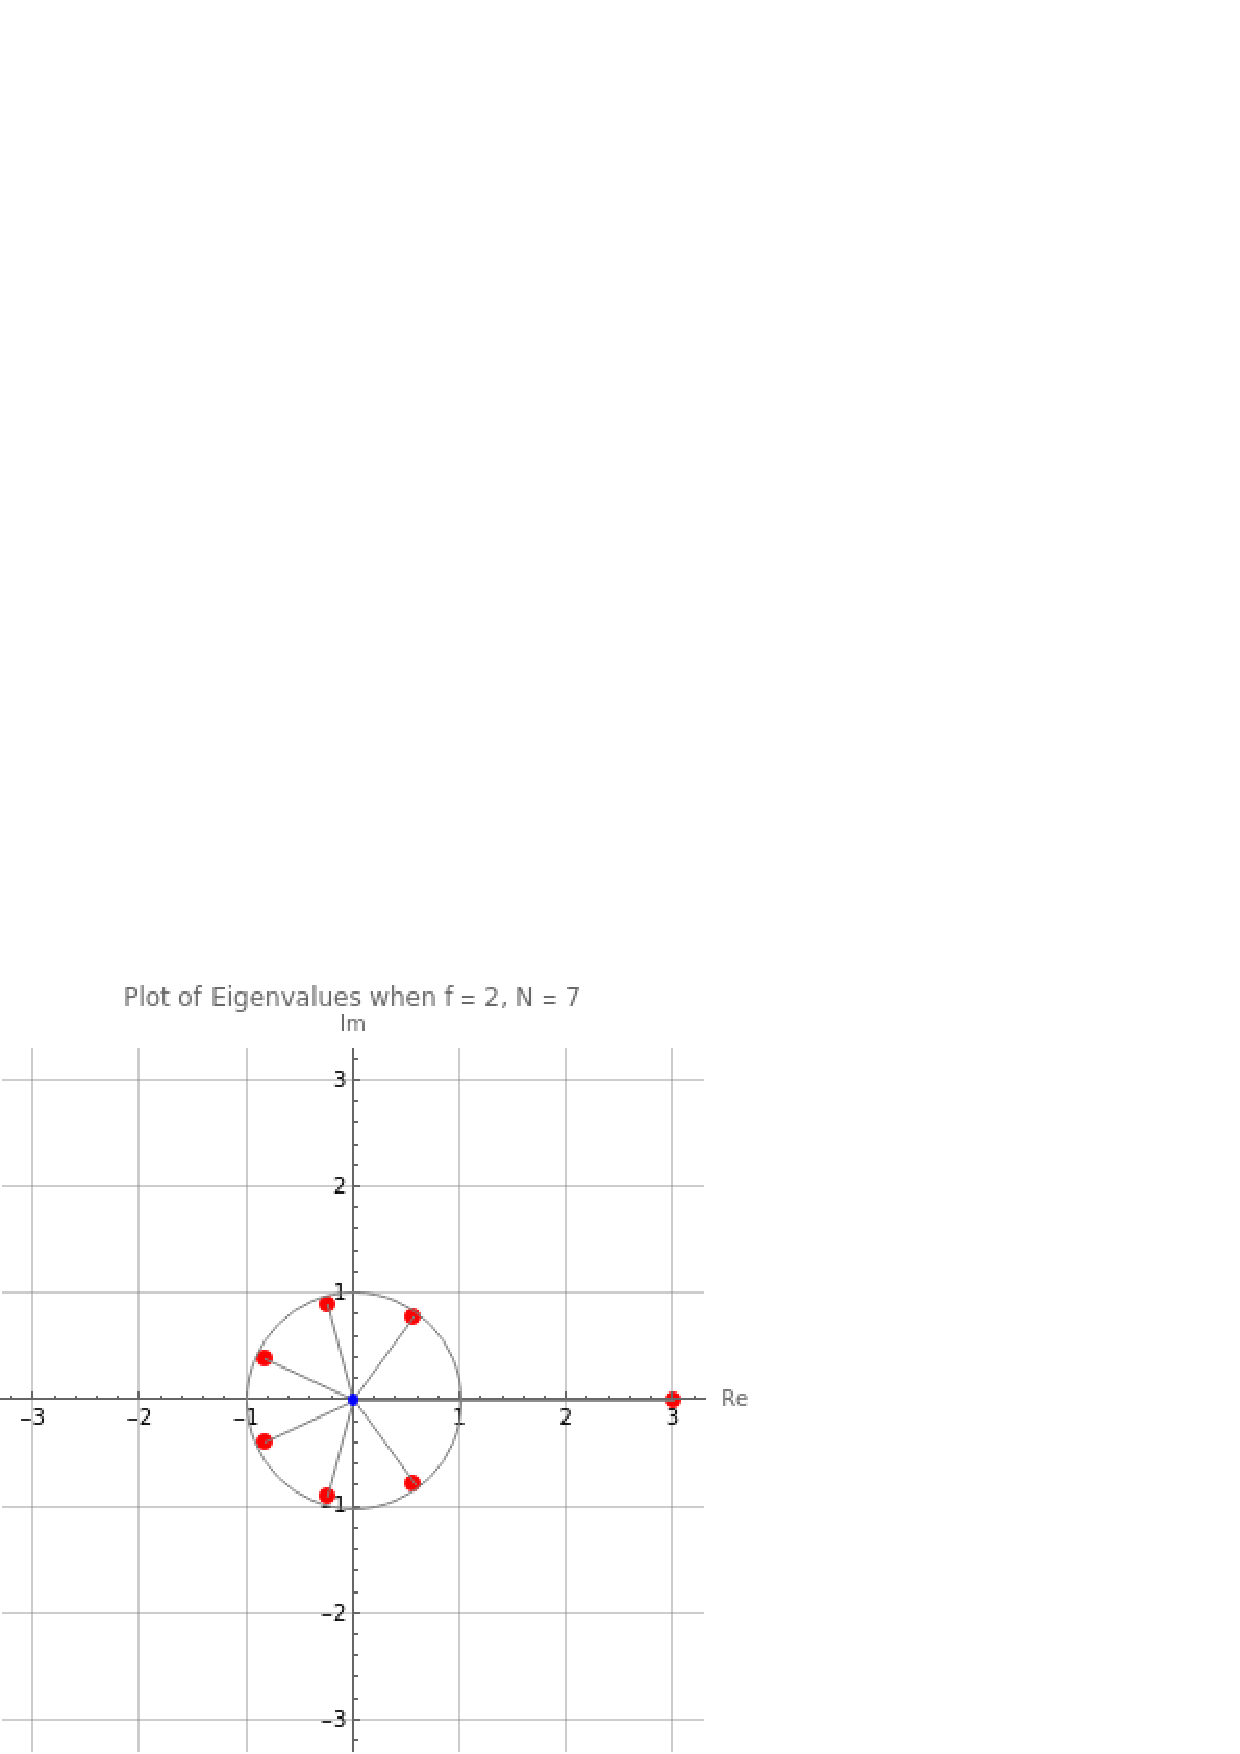
\includegraphics[width=\textwidth]{f2N7.png}
        \caption{$f > 1$, $N$ odd}
        \label{fig:fig1}
    \end{subfigure}
    \hfill
    \begin{subfigure}[b]{0.45\textwidth}
        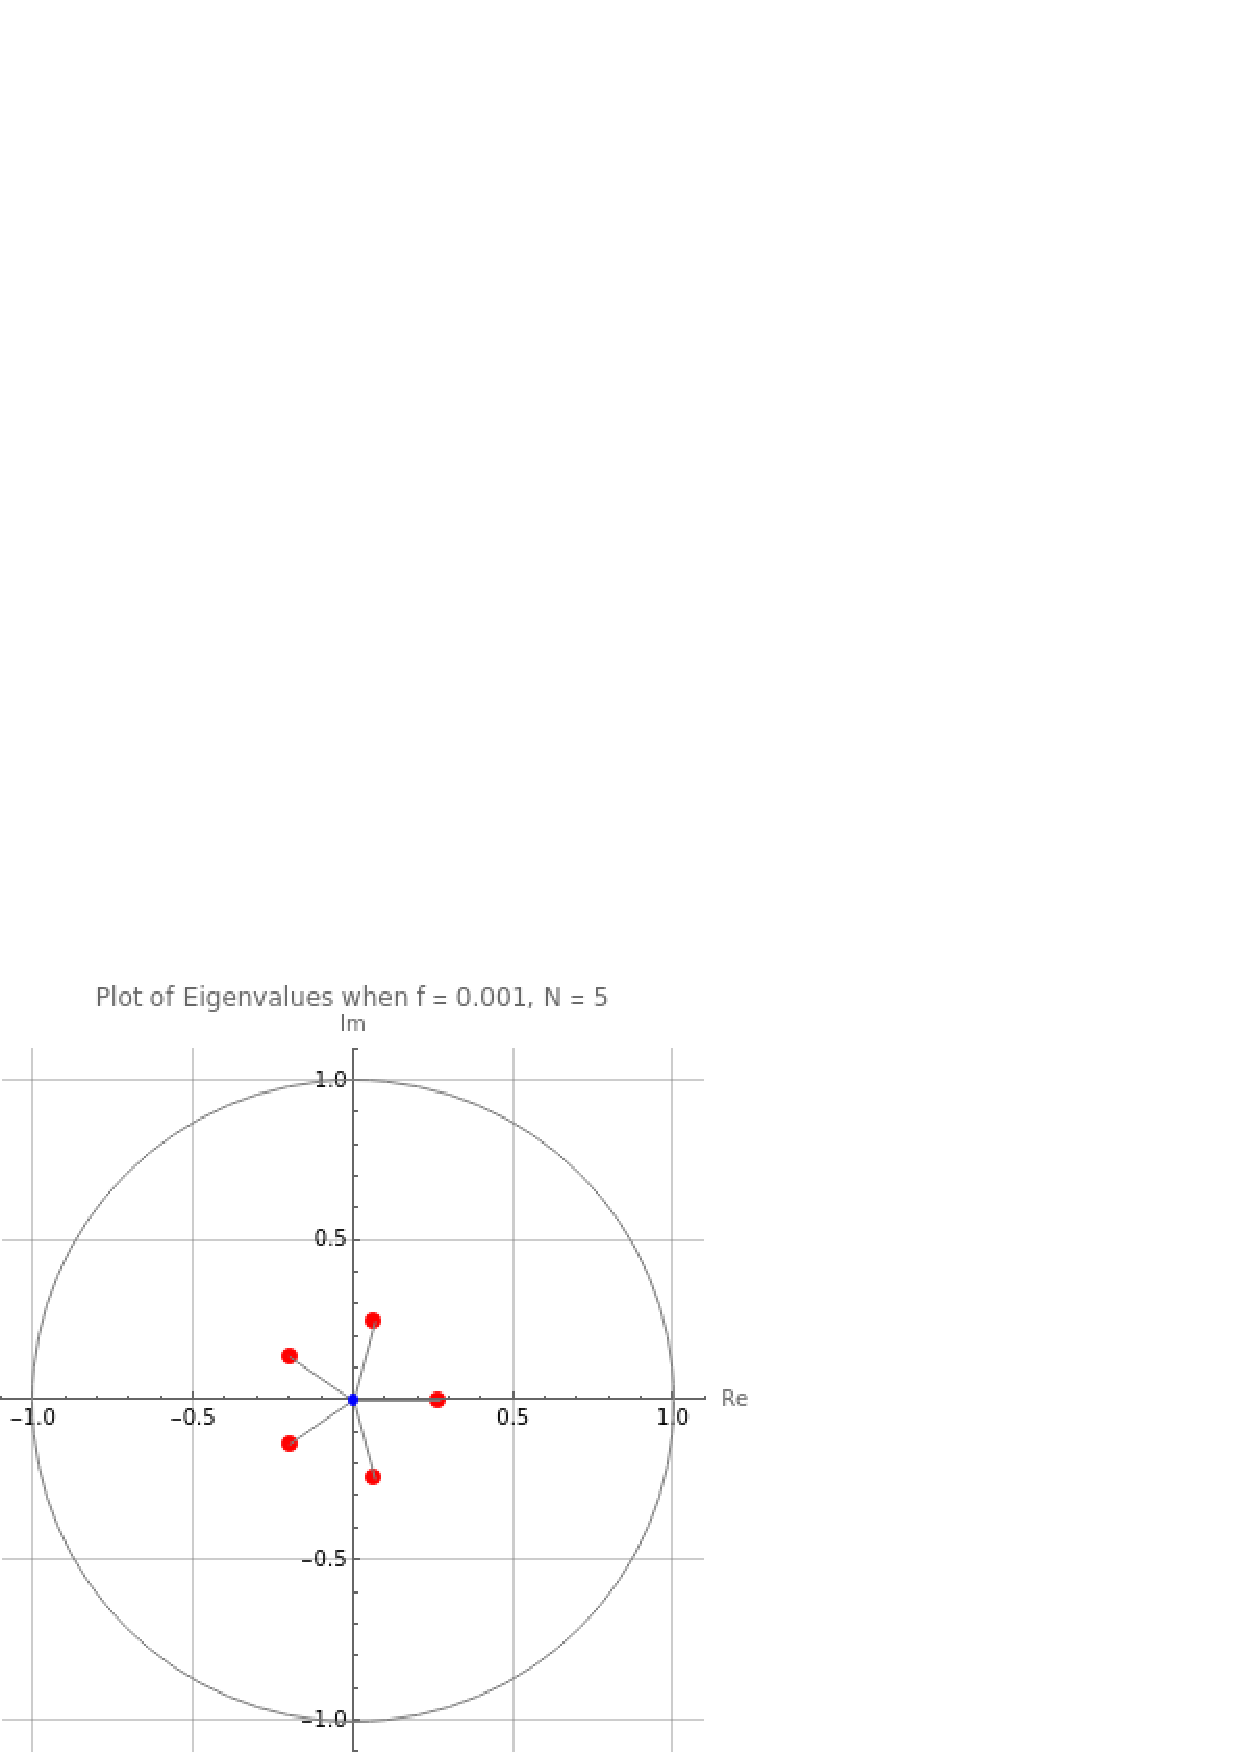
\includegraphics[width=\textwidth]{fsmN5.png}
        \caption{Small fertility rate}
        \label{fig:fig2}
    \end{subfigure}
    \\
    \begin{subfigure}[b]{0.45\textwidth}
        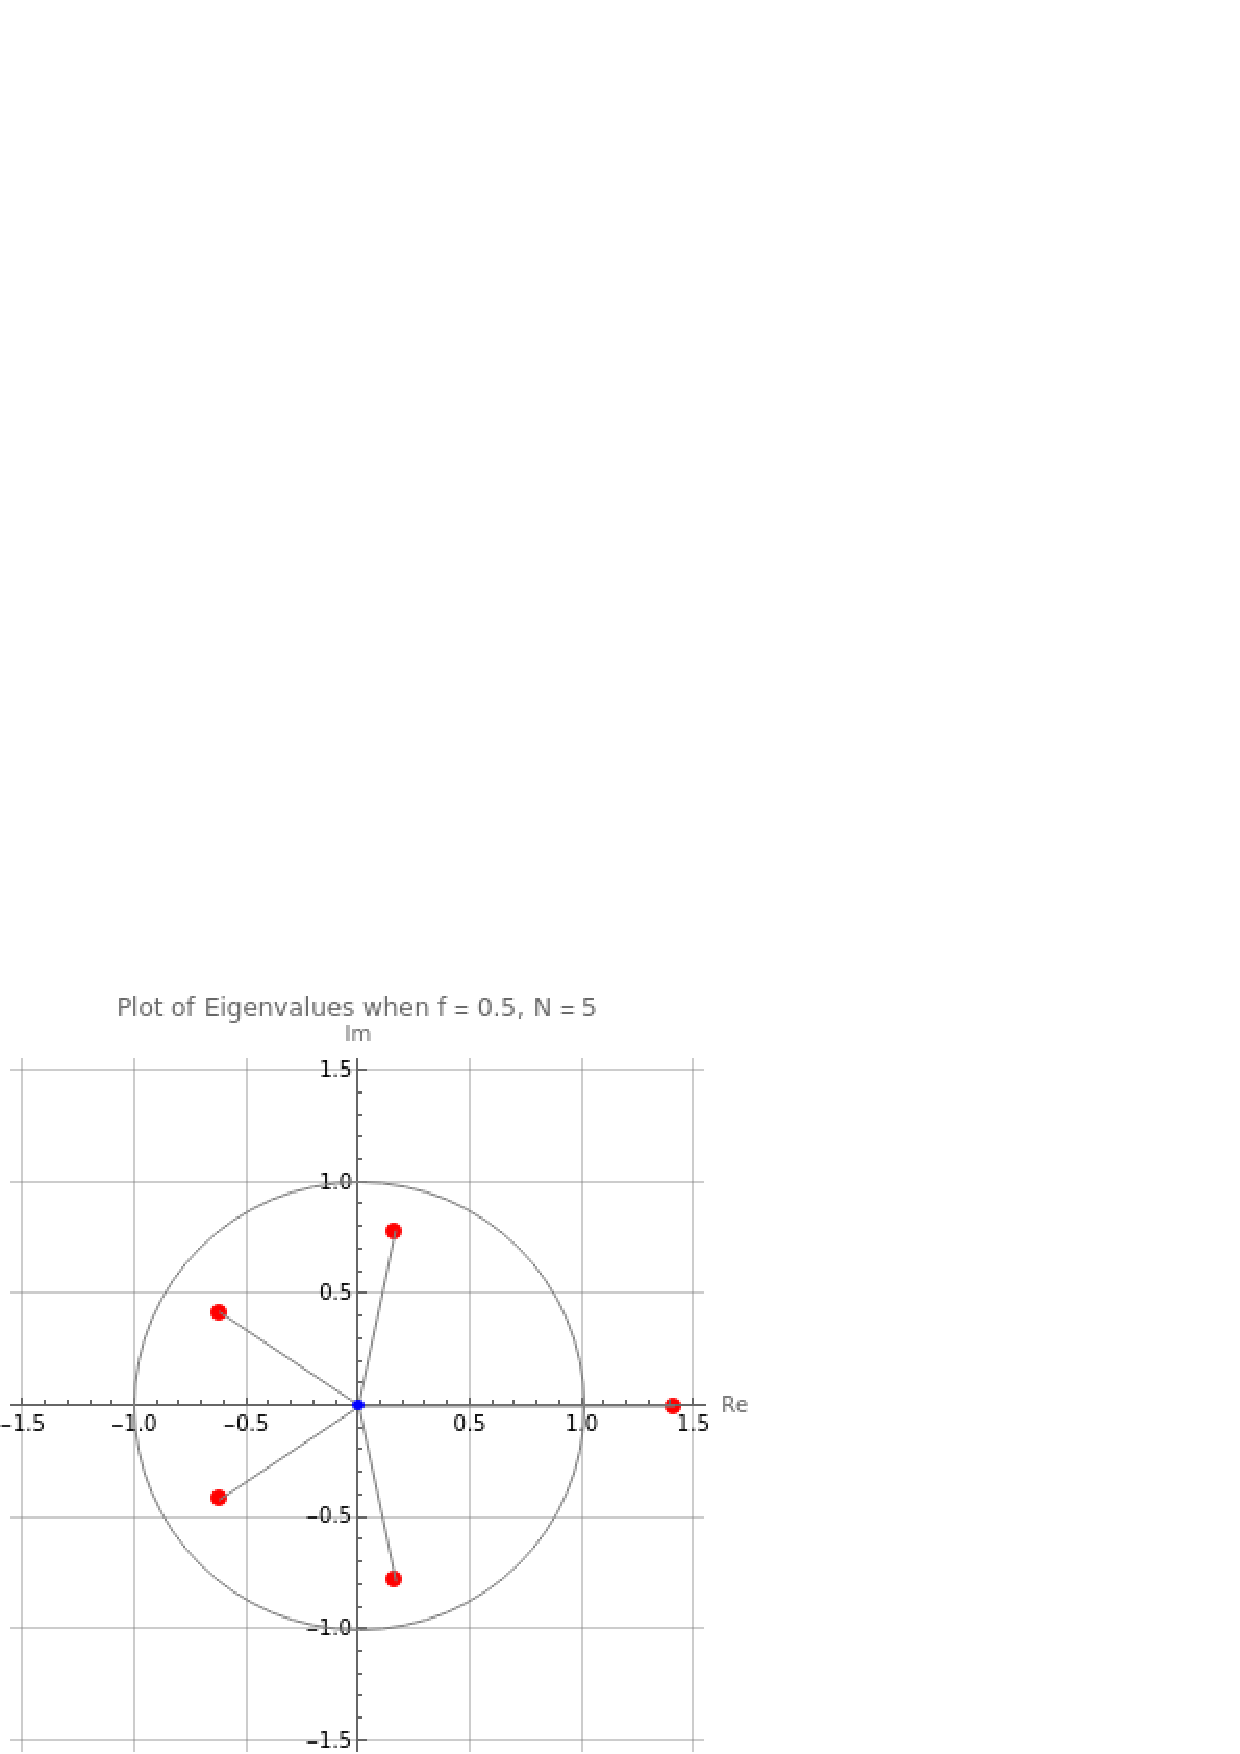
\includegraphics[width=\textwidth]{fHfN5.png}
        \caption{$f < 1$}
        \label{fig:fig3}
    \end{subfigure}
    \hfill
    \begin{subfigure}[b]{0.45\textwidth}
        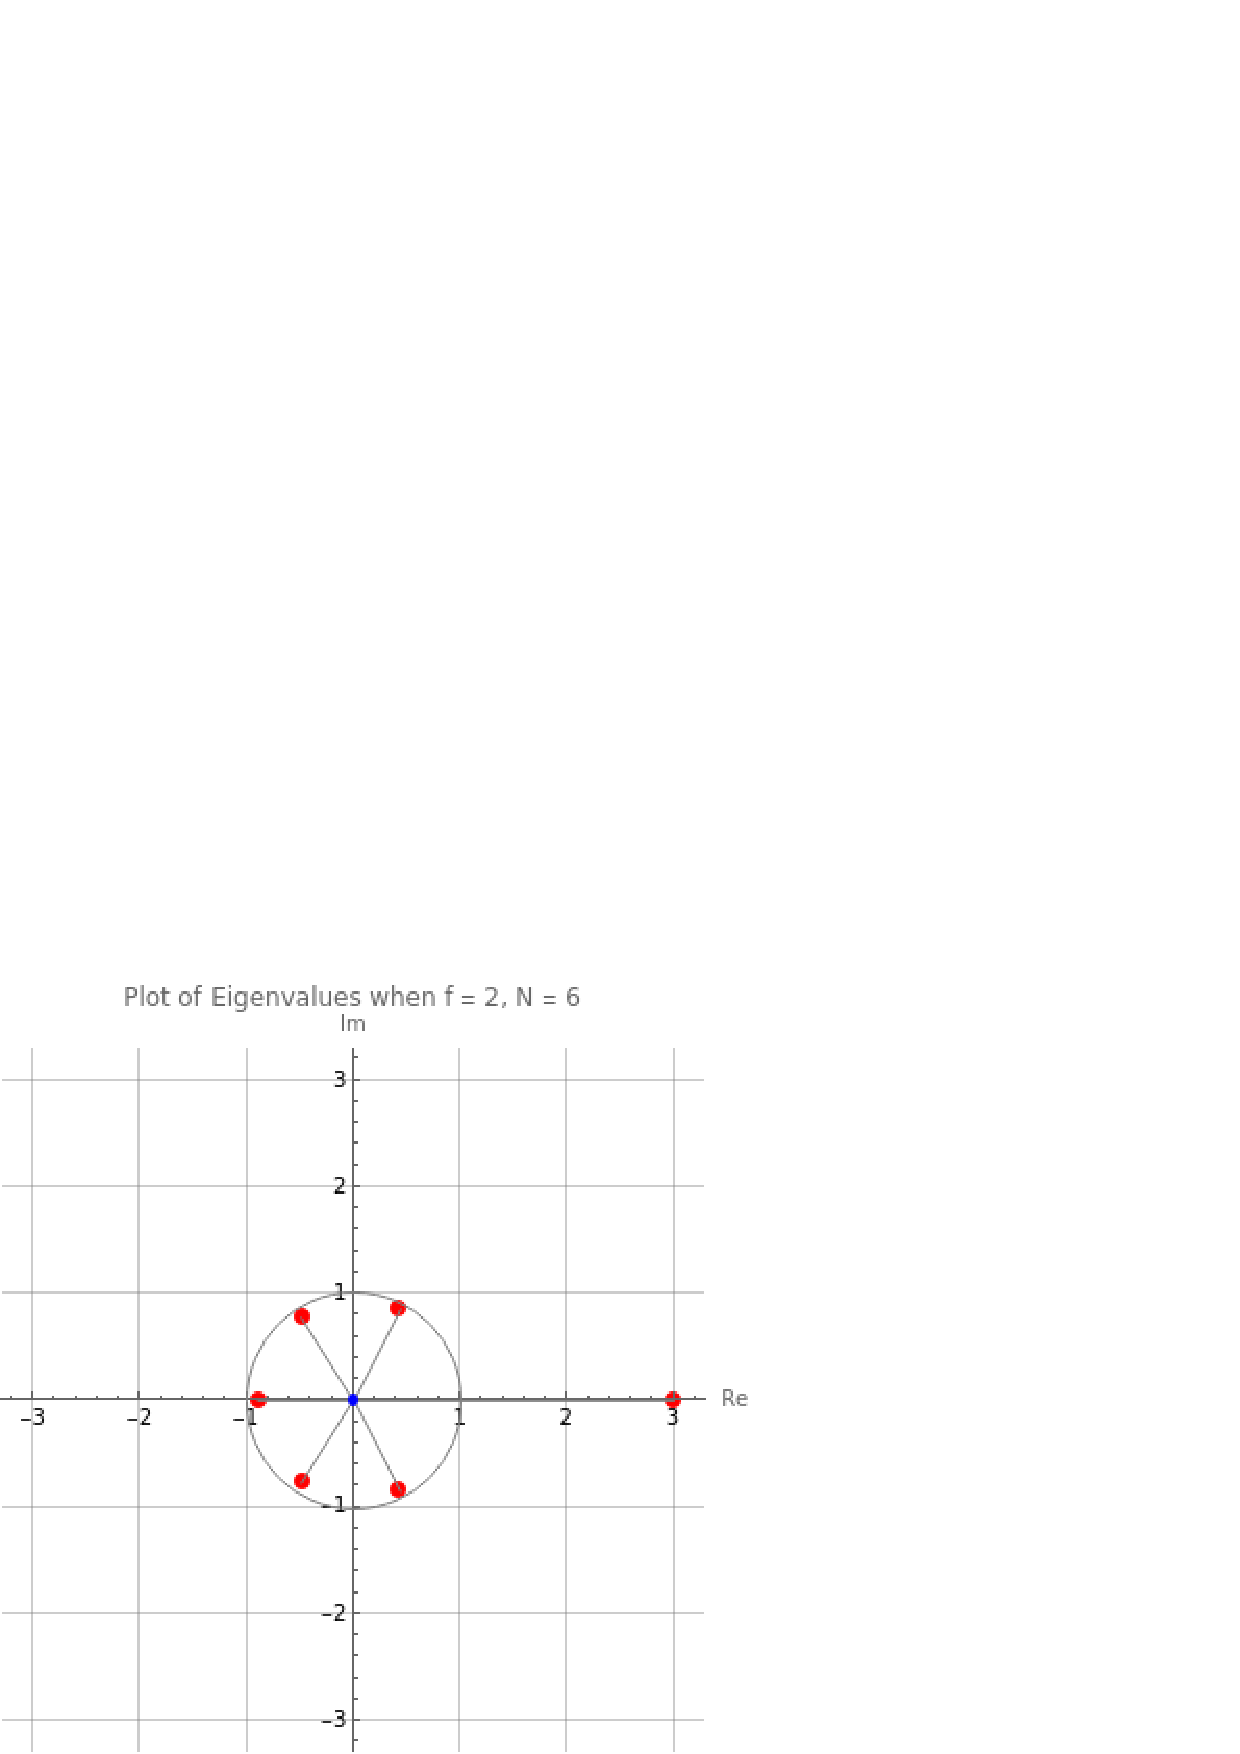
\includegraphics[width=\textwidth]{f2N6.png}
        \caption{$f > 1$, $N$ even}
        \label{fig:fig4}
    \end{subfigure}
    \caption{Complex Eigenvalues of Simple Leslie Matricies for varying $f, N$}
    \label{fig:overall}
\end{figure}

\newpage

\begin{cor}[Real Root of the Characteristic Equation]

    The real root of the characteristic equation has a magnitude greater 
    than $1$, if and only if $1-fN < 0$. 
\end{cor}
\begin{proof}
    We know that $\ch_(z)$ can be evaluated somewhere in 
    the interval $[1, \infty)$ to be positive. 
    Evaluate the following. 
    \[
        \ch_N(1) = 1 - fN
    \]
    If this value is less than zero, than the real 
    root lies somewhere in the range $(1, \infty)$. 
    Otherwise, since $f(0) < 0$, the dominant root 
    must be less than $1$. 
\end{proof}



With a little more analysis, we provide a lower bound and the 
upper bound of the maximum eigenvalues of $L_f$. 

\begin{theorem}[Bounds for the maximum eigenvalue]\label{thm:Bound}

 Given that $1-fN \leq 0$, the maximum eigenvalue of $L_f$ of order 
 $N$ is given by 
 \[
 1 + f - \frac 1 {N} \leq \lambda_{max} \leq 1 + f
 \]
\end{theorem}

\begin{proof}
    The upper bound is trivial. 
    \[
        \ch_N(1+f) \ = \ f > 0
    \]  
    $\ch_N(0) = -f < 0$ and by the intermediate value theorem, the maximum root is 
    bounded. 

    To obtain the lower bound, we write $f = 1/N + \epsilon$ for 
    some $\epsilon > 0$. With some algebra, we compute $\ch_N(z)$ at the lower 
    bound. If we show that this value is less than zero, the 
    dominating root must be greater than the purported lower bound. 
    \[
        \ch_N\left(
            1 + f - \frac 1 N
        \right)  \ = \ -
        \left(
            1 + f - \frac 1 N
        \right)^N \left[
            \frac {1} {fN - 1}
        \right]
        + \frac {fN} {fN - 1}
    \]
    We wish to bound this value under zero. It suffices to show 
    \[
        fN - \left(
            1 + f - \frac 1 N
        \right)^N < 0
    \]
    Which, using the $\epsilon$ substitution converts to 
    \[
        1 + N\epsilon - (1 + \epsilon)^N \ < \ 0
    \]
    And expanding the power term by the binomial theorem, 
    the inequality must hold. 
\end{proof}

\section{The predator-prey model}
%PP model
\subsection{The predator-prey model with Leslie Matricies}

\begin{definition}[Leslie Predator-Prey]
Let $\vec \alpha_n$, $\vec \beta_n$ be the population vectors 
of the predator and prey at timestep $n$. 
Set the number of age groups of both population to be 
$N$, so the population vectors will have entries. 
\begin{eqnarray}
    \vec \alpha_n \ = \ (\alpha_n^{(1)}, \dots, \alpha_n^{(N)}) 
    \nonumber \\
    \vec \beta_n \ = \ (\beta_n^{(1)}, \dots, \beta_n^{(N)}) 
\end{eqnarray}
 The population 
vectors are defined by the following 
system of matrix differences. 
\begin{eqnarray}
    \vec \alpha_{n - 1} &=& L_a \vec \alpha_n + k m \vec \beta_n \nonumber \\ 
    \vec \beta_{n - 1} &=& L_b \vec \beta_n - k \vec \alpha_n
\end{eqnarray}
$k, m$ are predation ratio and nurturing ratios, both greater than zero. 
We set the population of predator and prey to be the sum 
of all entries. In symbols, we write $P_{a, n}, P_{b, n}$ the population 
of the predator and prey by the following sums. 
\begin{equation}
    P_{a, n} \ = \ \sum_{k = 1}^{N} \alpha^{(k)}_{n}  
    \textAnd
    P_{b, n} \ = \ \sum_{k = 1}^{N} \beta^{(k)}_{n} 
\end{equation}
\end{definition}


We assume that the x-value of $L_\alpha$ is less than $1/2$ 
and that the x-value of $L_\beta$ is greater than $1/2$. In 
other words, the predator population decays in absense of the prey 
and the prey populatin explodes in absence of the predator. 
Moreover, the population is fixed to be nonnegative. 

If the population reaches zero 
at some time $n \in \mathbb{Z}_{pos}$, 
we say that the population has gone 
extinct. 
Notice that if the predation rate is too high, the prey population 
will be exhausted. In the absence of the prey, the predator 
population will be extinct. On the other hand, if the predation 
rate is too low, the predator population will not be able to maintain 
itself, and hence will go extinct. Hence, it is natural to ask 
the following question. 

\begin{question}[Optimal Predation Strategy]
For what ranges of the real value $k$ guarantees exponential growth 
of the predator? Moreover, what value of $k$ is necessary to guarantee 
maximum growth?
\end{question}

Furthermore the real-valued formula motivates us to introduce an 
extra factor of $i$ in the recurrence.  

\begin{definition}[Complex Predator-Prey]
Let $\alpha_n$, $\beta_n$ be the population vectors 
of the predator and prey at timestep $n$. The population 
vectors are defined by the following 
system of matrix differences. 


\begin{eqnarray}
    \vec \alpha_n \ = \ (\alpha_n^{(1)}, \dots, \alpha_n^{(N)}) 
    \nonumber \\
    \vec \beta_n \ = \ (\beta_n^{(1)}, \dots, \beta_n^{(N)}) 
\end{eqnarray}
 The population 
vectors are defined by the following 
system of matrix differences. 
\begin{eqnarray}
    \vec \alpha_{n - 1} &=& iL_a \vec \alpha_n + k m \vec \beta_n \nonumber \\ 
    \vec \beta_{n - 1} &=& iL_b \vec \beta_n - k \vec \alpha_n
\end{eqnarray}
$k, m$ are predation ratio and nurturing ratios, both greater than zero. 
We set the population of predator and prey to be the sum 
of all entries. In symbols, we write $P_{a, n}, P_{b, n}$ the population 
of the predator and prey by the following sums. 
\begin{equation}
    P_{a, n} \ = \ \left\|\sum_{k = 1}^{N} \alpha^{(k)}_{n} \right\|
    \textAnd
    P_{b, n} \ = \ \left\|\sum_{k = 1}^{N} \beta^{(k)}_{n} \right\|
\end{equation}
\end{definition}

Experimentally speaking, for the complex model, the population 
grows almost surely unless the predation rate $k$ is zero. The natural 
question to ask for this model is the following. 

\begin{question}[Modeling Predator Growth]
    What is the growth rate of the predator as $n \rightarrow \infty$
\end{question}

%Might add the winner-takes all thm?

By elementary substitutions, we obtain the follwoing proposition. 

\begin{prop}[Coupled 1st order to 2nd order]\label{thm:to2ndOrd}
Assuming both 
the prey and predator population are nonextinct within 
a given period of time, 
the predator population satisfies the following second order 
difference equation. 
\begin{eqnarray}
\alpha_n = (L_a + L_b) \alpha_{n - 1} - L_b L_a \alpha_{n -2} - m k^2 \alpha_{n - 2} \nonumber
\\
\beta_n = (L_b + L_a) \beta_{n - 1} - L_a L_b \beta_{n -2} - m k^2 \beta_{n - 2}
\end{eqnarray}
For the complex model, 
\begin{eqnarray}
\alpha_n = i(L_a + L_b) \alpha_{n - 1} + L_b L_a \alpha_{n -2} - m k^2 \alpha_{n - 2} \nonumber
\\
\beta_n = i(L_b + L_a) \beta_{n - 1} + L_a L_b \beta_{n -2} - m k^2 \beta_{n - 2}
\end{eqnarray}
\end{prop}. 


The coupled second order difference equation can be solved using 
generating function under the assumption that the leslie matricies 
of the two populations are constant multiples of each other. 

\begin{theorem} [Generating Function of the predator population for real case]
    Suppose $\vec \alpha_n$ is the population vector 
    of the predator in a real Leslie Predator-Prey model where 
    $L = \rho L$ and $L_b = L$. 
    The generating function of $\vec \alpha_n$ is
    \begin{equation}
        G(x) \ = \ 
\frac{ \left(\rho L + m k^2 - (\rho + 1) L x\right)\vec \alpha_0 + (\rho L + m k^2) x \vec  \alpha_1}{x^2 - x(\rho + 1) L + \rho L^2 + m k^2}
    \end{equation}
\end{theorem}

\begin{proof}
    From the recurrence relation provided in proposition \ref{thm:to2ndOrd}, 
    we have the following identity. 
    \begin{equation}
        \begin{split}
        \left[x^2 - x (\rho + 1) L + (\rho L^2 + mk^2)\right]G(x) \\ = \  
        -(\rho + 1) L \vec \alpha_0 x 
        +(\rho L^2 + mk^2) \vec \alpha_0 
        + (\rho L^2  + m k^2) \vec \alpha_1 x
        \end{split}
    \end{equation}
    This identity can be verified by substituting $G(x)$ and 
    imposing the conditions on $\alpha_n$. The expansion on the 
    lefthand side has residues for terms that have a $x$ power 
    less than or equal to 2. Solve for $G(x)$ to obtain the result. 
\end{proof}


Using partial fraction decomposition, it is possible to obtain 
a closed form expansion for $\vec \alpha_n$. 

\begin{theorem} [Formula for $\vec \alpha_n$]
    For $\vec \alpha_n$ where $n > 0$, 
    \begin{equation}
    \vec \alpha_n \ = \ 
    \frac {
(L^2 \rho + k^2 m)^{n - 2}
    } {\sqrt D} 
    \left[
        \left(
            (k^2m + L^2 \rho) \vec \alpha_1 - L(1 + \rho) 
\left(
            k^2m + L^2\rho
        \right)
            \vec \alpha_0
        \right)\delta_{n - 1}
        + \left(
            k^2m + L^2\rho
        \right)^2\vec \alpha_0 \delta_{n}
    \right]
    \end{equation}
    where $D$ is defined as
    \begin{equation}
        D \ = \ L ^2 (1 + \rho)^2 - 4 (mk^2 + \rho L^2)
    \end{equation}
    and sequence $\delta_n$ defined as 
    \begin{equation}
        \delta_n \ = \ 
        \left(
            \frac 1 2
        \right)^n 
        \left(
            \frac 1 {
                L^2 \rho + k^2 m
            }
        \right)^{n}
        \left[
            \sum_{\substack{l = 1 \\ l \textnormal{ odd}}}^{n + 1}
            \binom{n + 1}{l} 
            [L(1+\rho)]^{t + 1 - l}(\sqrt D)^l
        \right]
    \end{equation}
\end{theorem}

\begin{proof}
    The derivation follows by applying partial fraction decomposition on the 
    Generating Function. 
\end{proof}

Though the theorem gives a closed-form equation for the population, 
the complexity of the formula poses difficulties to determine 
predation 

\subsection{Real-valued model where $L$ is a scalar}
%solution for scalars


The following three propositions properly models 
the population where the dimension of the Leslie matrix 
is 1. That is, the population growth is characterized 
by a exponential of a scalar without interaction. 
To emphasize the scalarness, write $l_a < 1$ and $l_b > 1$ 
instead of $L_a, L_b$. 

\begin{theorem}[Eigenvalues of the companion matrix]\label{thm:simpleEval}
Using proposition (\ref{thm:to2ndOrd}), it is possible to obtain a companion matrix that 
describes the population. 
\[
    \twobytwoMat(
        l_a + l_b, -l_a l_b -k^2 m, 1, 0
    )
\]
The eigenvalue of this matrix is purely real if and only if 
\begin{equation}
    k \leq \frac {l_a - l_b} {2\sqrt{m}}
\end{equation}
Otherwise, the eigenvalues of these maticies are complex conjugates 
of each other. 
\end{theorem}

\begin{proof}
    The coefficient matrix of the companion matrix is 
    \[
        \lambda ^2 - (l_a + l_b) \lambda + k^2m + l_a l_b
    \].
    The discriminant of this polynomial must be a nonnegative value. 
    In symbols, 
    \begin{equation}
        \frac D 4 \ =\ \frac {(l_a + l_b)^2} 4 - k^2m + l_a l_b \ \geq \ 0
    \end{equation}
    With elementary algebra, we obtain 
    \begin{equation}
    k \leq \frac {l_a - l_b} {2\sqrt{m}}
    \end{equation}
\end{proof}



\begin{theorem}[Exponential growth of population for small predation]
The following condition guarantees that the predator and prey population 
to not vanish as $n \rightarrow \infty$. 
\begin{equation}
    k \ \leq \ \sqrt{
        \frac {(1 - l_b)(l_a - 1)} {m}
    }
\end{equation}
\end{theorem}

\begin{proof}
    Assume that the discriminant is a nonnegative real value. Then, 
    the maximum eigenvalue must be 
    \[
        \frac {l_a + l_b} 2 + \frac {\sqrt D} 2
    \]
    which must be greater or equal to 1 for the population to not vanish. 
\end{proof}

\begin{theorem}[Complex eigenvalue implies extinction]
If 
\begin{equation}\label{eqn:simpleVanish}
    k \ > \  \frac {l_a - l_b} {2\sqrt{m}}
\end{equation}
then the population is guaranteed to be extinct. 
\end{theorem}
\begin{proof}
    It follows trivially that the condition (\ref{eqn:simpleVanish}) 
    implies that the eigenvalue is complex. Consider 
    powers of the complex eigenvalues as rotation along the complex 
    plane. There exists some arbitrary rotation that guarantees 
    the real part of the power to be negative. 
\end{proof}
\hfill \qed

\subsection{The Complex-valued model with $L_a = \rho L_b$}
%Special solution for leslie matricies

To solve the second order matrix 
recurrence related to 
the predator-prey model, 
we solve a characteristic equation 
where the coefficients are matricies. 
Since the only matricies involved on this equation are $I$ and $L_\beta$
which commute, we can use the quadratic equation to solve this equation. 


\begin{theorem}[Maximum Eigenvalue for the general case]\label{eqn:MaxEvalGen}
    The population vector of the predator in (\ref{LeslieDef}) 
    can be characterized as 
    \begin{equation}
    \vec \alpha_n =\Lambda_1^{n}  \vec v_1+ \Lambda_2^{n}\vec v_2
    \end{equation}
    for some vectors $\vec v_1$ and $\vec v_2$. The 
    growth of the predator population 
    is dominated by the maximum eigenvalue 
    of $\Lambda_1$. Call the maximum eigenvalue of $L_b$ 
    as $\lambda_{max}$. Then, the maximum eigenvalue of $\Lambda_1$, 
    denoted by $\Lambda_{max}$ has the following modullus. 
    \begin{equation}
        \|\Lambda_{max} \| \ =\   \frac {
            (\rho + 1)\lambda_{max} + \sqrt{(\rho + 1)^2 \lambda_{max}^2 + 4mk^2}
        } 2
    \end{equation}. 
\end{theorem}
\begin{proof}
    It is possible to solve for $\Lambda_1, \Lambda_2$ directly. 
We wish to find a matrix $\Lambda$ such that 
\begin{equation}
\Lambda^2 - i(\rho + 1) L_b \Lambda + \rho L_b^2+ mk^2 I = 0
\end{equation}
    Apply the quadratic formula. 
    \begin{eqnarray}
        \Lambda_1 \ = \ 
        \frac {
        (1 + \rho) L_b^2 + 
        \sqrt{
        (1-\rho)^2L_b^2 + mk^2
        }
        } 2 i \nonumber \\ 
 \Lambda_2 \ = \ 
        \frac {
        (1 + \rho) L_b^2 - 
        \sqrt{
        (1-\rho)^2L_b^2 + mk^2
        }
        } 2 i
    \end{eqnarray}
    The magnitude of $\Lambda_1$ is greater than that of $\Lambda_2$. 
    We approximate the population of the predator at the limit $n \rightarrow \infty$. 
    \begin{eqnarray}
        P_{a, n} \ = \ \|\vec a_n\| \ = \ 
        \|\Lambda_1\|^n \|\vec v_1\| + 
 \|\Lambda_2\|^n \|\vec v_2\| 
 \ \approx  \ 
\|\Lambda_1\|^n \|\vec v_1\|
    \end{eqnarray}
\end{proof}

With some more analysis, we provide a bound for $k$ that guarantees 
the survival of both the predator and $k$.

\begin{comment}

\begin{theorem}
    Given that $\rho \ \geq \ \frac {-f + 1/N} {2 + f - 1/N}$, the following condition 
    guarantees population growth. 
 \begin{equation}\label{eqn:finalBound}
        k \ \leq \  \frac{
            \sqrt{(\rho + 1)^2(1 + f - 1/N)^2 - (1 - \rho)^2}
        }{2\sqrt{m}}
    \end{equation}
\end{theorem}

\begin{proof}
    We proceed with multiple inequality, and provide conditions 
    to guarantee that the bounds are purely real. 
    Using theorem (\ref{thm:Bound}), we recognize a following 
    lower bound for $\Lambda_1$. 
    \begin{equation}
        \Lambda_1 \ \geq \ 
 \frac {
            (\rho + 1) + \sqrt{(\rho + 1)^2 (1 + f - 1/N)^2 - 4mk^2}
        } 2
    \end{equation}
    The value inside the square root must be nonnegative. Hence, 
    we end up with the condition 
    \begin{equation}\label{eqn:intermediateBound}
        k \ \leq \ \frac{(\rho + 1) (1 + f - 1/N)} {2 \sqrt m}
    \end{equation}
    We set the righthand side to be greater or equal to 1. 
    With some algebra, we deduce the condition 
    \begin{equation}\label{eqn:finalBound}
        k \ \leq \  \frac{
            \sqrt{(\rho + 1)^2(1 + f - 1/N)^2 - (1 - \rho)^2}
        }{2\sqrt{m}}
    \end{equation}
    and we notice that this condition is stronger than (\ref{eqn:intermediateBound})
    It finally remains to confirm that the final upper bound is indeed real. 
    Take term inside the square root of (\ref{eqn:finalBound}) and set it to be greater than or 
    equal to 
    zero, and this yields the following. 
    \begin{equation}
        \rho \ \geq \ \frac {-f + 1/N} {2 + f - 1/N}
    \end{equation}
\end{proof}



\begin{remark}
    Under the substitution 
    \begin{gather}
        \phi \ = \ 
 \frac{
            \sqrt{(\rho + 1)^2(1 + f - 1/N)^2 - (1 - \rho)^2}
        }{2\sqrt{m}}
        \nonumber \\
        \varphi \ = \  \frac {-f + 1/N} {2 + f - 1/N}
    \end{gather}
    the growth condition simplifies to 
    \begin{eqnarray}
        k \ \leq \ \phi \textAnd \rho \ \geq \ \varphi
    \end{eqnarray}
\end{remark}

\begin{figure}[htp]
    \centering
    \begin{subfigure}[b]{0.45\textwidth}
        \includegraphics[width=\textwidth]{kprv1.png}
        \label{fig:fig1}
    \end{subfigure}
    \hfill
    \begin{subfigure}[b]{0.45\textwidth}
        \includegraphics[width=\textwidth]{kprv2.png}
        \label{fig:fig2}
    \end{subfigure}
    \
    \begin{subfigure}[b]{0.45\textwidth}
        \includegraphics[width=\textwidth]{kprv_cap1.png}
        \caption{Growth condition unsatisfied}
        \label{fig:fig3}
    \end{subfigure}
    \hfill
    \begin{subfigure}[b]{0.45\textwidth}
        \includegraphics[width=\textwidth]{kprv_cap2.png}
        \caption{Growth condition satisfied}
        \label{fig:fig4}
    \end{subfigure}
    \caption{Predator Prey model with different parameters}
    \label{fig:overall}
\end{figure}



\begin{remark}
    The growth condition is a sufficient but not necessary condition 
    for population growth. We provide a case where the growth condition 
    is unsatisfied but the predator population grows exponentially. 
\end{remark}

\begin{figure}[htp]
    \centering
    \includegraphics[width=0.8\textwidth]{kprv3.png} 
    \includegraphics[width=0.8\textwidth]{kprv_cap3.png} 
    \caption{Counterexample: expnential growth without growth condition}
    \label{fig:example}
\end{figure}

\newpage


\end{comment}

\section{The Competetive Model}
We can slightly modify one of the sign of the model and 
study the following system. Suppose there exists two identical 
population that has a same growth matrix $L$. Also, assume 
that the population is nonvanishing without interaction. That is, 
$\lambda_{max}$, the maximum eigenvalue of $L$ is greater 
than or equal to 1. 
\begin{definition}[Leslie Competetive Model]
Let $\alpha_n$, $\beta_n$ be the population vectors 
of the predator and prey at timestep $n$. The competetive 
model is defined by the following 
system of matrix differences. 
\begin{eqnarray}\label{eqn:conditions}
    \alpha_{n + 1} &=& \max(L \alpha_n - k m \beta_n, \vec 0) \\ 
    \beta_{n + 1} &=& \max(L \beta_n - k \alpha_n, \vec 0) \nonumber
\end{eqnarray}
$k, m$ are interaction ratio and competetive advantage, both between $0, 1$. 
\end{definition}


\subsection{Last Species Standing}

A similar analysis used for the predator-prey model 
can be applied to yield the following result. 

\begin{theorem}[Last Species Standing]
    Suppose $\vec \alpha_0 = \alpha_0 (1, \cdots, 1)$ and 
    $\vec \beta_0 = \beta_0 (1, \cdots, 1)$.
    In a Leslie competetive model, one of the two 
    species are likely to vanish as $n \rightarrow \infty$  
    The fate of the species is determined 
    by the sign of the term 
    \[
        D := \alpha_0 - \sqrt{m} \beta_0
    \]
    . To qualify, if $D > 0$, then the population $\alpha$ 
    vanishes and population $\beta$ grows exponentially.
     If $D < 0$, then the population $\beta$ vanishes and the population $\alpha$ 
     grows exponentially. 
    If $D = 0$, either both species vanish or grow exponentially together. 
\end{theorem}

\begin{proof}
    Proposition (\ref{thm:to2ndOrd}) can be simply generalized by 
    the substitution \newline $m \mapsto -m$. From the recursive relation 
    \begin{equation}
        \alpha_n \ = \ (2L)\alpha_{n - 1} -L^2 \alpha_{n - 2} + mk^2 \alpha_{n - 2}
    \end{equation}
    we obtain the characteristic eqation 
    \begin{equation}
    \Lambda ^2 - 2L \Lambda + L^2 - mk^2 \ =\ 0
    \end{equation}
    and by the quadratic formula, we derive the root. 
    \begin{equation}
        \Lambda_1 \ = \ L + k\sqrt{m} I \textAnd \Lambda_2\ = \ L - k\sqrt{m} I
    \end{equation}
    $I$ is the identity matrix. 
    Notice that $k, m$ are both nonnegative real values, and $L$ 
    is assumed to guarantee positive population growth. Hence, 
    $\Lambda_1$ has a positive eigenvalue. 

    From (\ref{eqn:MaxEvalGen}), we characterize the population as
    \begin{equation}\label{eqn:closedEq}
    \vec \alpha_n \ =\ \Lambda_1^{n}  \vec v_1+ \Lambda_2^{n}\vec v_2
    \end{equation}
    In the far limit, as $n \rightarrow \infty$, 
    \begin{equation}
    \vec \alpha_n \ \approx\ \Lambda_1^{n}  \vec v_1
    \end{equation}
    Thus, the population is nonvanishing if and only if $\vec v_1$ 
    is positive. Compute $\vec v_1$ directly. We have the following conditions 
    from (\ref{eqn:closedEq}), we obtain two conditions. 
    \begin{eqnarray}
        \vec \alpha_0 \ = \ \vec v_1 + \vec v_2 \nonumber \\ 
        \vec \alpha_1 \ = \ \Lambda_1 \vec v_1 + \Lambda_2 \vec v_2
    \end{eqnarray}
    Solving for $\vec v_1$, obtain 
    \begin{equation}
        \begin{split}
        \vec v_1 \ = \ \frac {\Lambda_2 \vec\alpha_0 - \vec\alpha_1} {\Lambda_2 - \Lambda_1}
        \ = \ 
        \frac {L\vec \alpha_0 - k\sqrt m \vec \alpha_0 - L \vec \alpha_0 + km\beta_0} {2mk} 
        \ = \ 
        \frac {\sqrt{m}\vec\beta_0 -  \vec \alpha_0} {2\sqrt m} \\ 
        \ = \ \frac {\sqrt m \beta_0 - \alpha_0} {2 \sqrt m} (1, \dots, 1) 
        \ = \ -\frac D{2\sqrt m} (1, \dots, 1) 
        \end{split}
    \end{equation}
    Similarly, we obtain 
    \begin{equation}
        \beta_n \ \approx \ \Lambda_1 \vec w_1  
    \end{equation}
    where 
    \begin{equation}
        \vec w_1 \ = \ \frac{\alpha_0 - \sqrt m \beta_0} {2 \sqrt m} (1, \dots, 1)
        \ = \ \frac D {2\sqrt m }(1, \dots, 1)
    \end{equation}
    . If $D \neq 0$, plugging in the appropriate value of $D$ yields 
    the result. Suppose $D = 0$ or $\alpha_0 = \sqrt m \beta _0$. The 
    conditions of (\ref{eqn:conditions}) imply the following. 
    \begin{eqnarray}
        \vec \alpha_1  \ = \ L \vec \alpha_0 - k \sqrt m \vec \alpha_0 \nonumber \\ 
        \vec \beta_1 \ = \ L \vec \beta_0 - k \sqrt m \vec \beta_0
    \end{eqnarray} 
    By induction, it is possible to prove that 
    \begin{eqnarray}
        \vec \alpha_n \ = \ \sqrt m \vec \beta_n
    \end{eqnarray}
    for all nonnegative integers $n$. In turn, we obtain 
    \begin{eqnarray}
        \vec \alpha_{n + 1} \ = \ 
        \left(
            L - k \sqrt m
        \right)^n \vec \alpha_0 \nonumber
        \\ 
        \vec \beta_{n + 1} \ = \ 
        \left(
            L - k \sqrt m
        \right)^n \vec \beta_0
    \end{eqnarray}
    and the population grows or vanishes simultaneously. 
\end{proof}


\begin{comment}
\section{Difficulties for the general case solution}
%Fuuture works


It turns out that solving the recurrence for the general case 
where $L_a, L_b$ is extremely challenging. Suppose we wish to 
solve the PP model where the Leslie matricies are degree $k$-by-$k$, 
where $k > 1$. If we adopt the scalar solution, we have to compute 
the eigenvalues of a $2k$-by-$2k$ matrix, and show that the eigenvector 
corresponding to the dominating eigenvalue is positive. Another 
attempted solution was to consider the following characteristic equation of 
the 2nd order recurrence
\[
    \Lambda^2 - (L_\alpha + L_\beta) \Lambda + (L_\alpha L_\beta - k^2 m I) = 0
\]
In general, $L_\alpha$ and $L_\beta$ do not commute. This imposes 
hardships when applying the quadratic formula to solve this equation.
\end{comment}



\printbibliography

\end{document}